\documentclass[UTF8,a4paper,12pt,openany]{ctexbook}
\newcommand{\ReportTitle}{具身智能行业和技术发展调研报告}
\newcommand{\ReportVersion}{v0.2}
\newcommand{\ReportAuthor}{个人学习与研究用途}

\newcommand{\ReportBibStyle}{gb7714-2015}
\usepackage{geometry}
\geometry{a4paper, left=28mm, right=28mm, top=25mm, bottom=25mm, headheight=15pt}

\usepackage{amsmath,amssymb,mathtools}
\usepackage{graphicx}
\usepackage{booktabs}
\usepackage{array}
\usepackage{longtable}
\usepackage{tabularx}
\usepackage{xltabular}
\usepackage{adjustbox}
\usepackage{enumitem}
\usepackage{float}
\usepackage{xcolor}
\usepackage{listings}
\usepackage{caption}
\usepackage{newunicodechar}
\usepackage{hyperref}
\usepackage{url}
\providecommand{\ReportBibStyle}{authoryear}
\usepackage[backend=biber,style=\ReportBibStyle]{biblatex}
\addbibresource{references/references.bib}
\AtBeginBibliography{\raggedright}

\setCJKmainfont{FangSong}[AutoFakeBold=0.2,AutoFakeSlant=0.15]
\setCJKsansfont{SimHei}
\setCJKmonofont{FangSong}
\setmainfont{FangSong}[AutoFakeBold=0.2,AutoFakeSlant=0.15]
\setsansfont{SimHei}
\setmonofont{FangSong}
\newunicodechar{•}{\ensuremath{\bullet}}

\hypersetup{
  colorlinks=true,
  linkcolor=black,
  urlcolor=blue,
  citecolor=black,
  pdftitle={\ReportTitle-\ReportVersion},
  pdfauthor={\ReportAuthor}
}

\setlist[itemize]{leftmargin=2em, itemsep=2pt, topsep=4pt}
\setlist[enumerate]{leftmargin=2em, itemsep=2pt, topsep=4pt}
\renewcommand{\labelitemi}{$\bullet$}
\renewcommand{\labelitemii}{$\circ$}
\setlength{\parindent}{2em}
\setlength{\parskip}{0.35em}
\setlength{\emergencystretch}{3em}
\raggedbottom
\linespread{1.25}

% The 27 report parts are the page-level divisions. Numeric chapters and
% subsections remain in the current page flow unless natural pagination occurs.
\newcommand{\reportpart}[1]{%
  \clearpage
  \phantomsection
  \noindent{\fontsize{18pt}{24pt}\selectfont\bfseries #1\par}%
  \medskip
}

\lstset{
  basicstyle=\small\ttfamily,
  breaklines=true,
  breakatwhitespace=false,
  columns=fullflexible,
  frame=single,
  keepspaces=true,
  showstringspaces=false,
  numbers=left,
  numbersep=8pt,
  xleftmargin=2em,
  literate={π}{{$\pi$}}1 {Δ}{{$\Delta$}}1 {≈}{{$\approx$}}1 {×}{{$\times$}}1
}

\newcolumntype{Y}{>{\raggedright\arraybackslash}X}
\graphicspath{{figures/}{../../../../assets/images/}{../../../../assets/diagrams/}}

\newcommand{\evidencefact}[1]{\par\noindent\textbf{证据事实：}#1\par}
\newcommand{\authorjudgement}[1]{\par\noindent\colorbox{black!6}{\parbox{0.94\linewidth}{\textbf{综述判断：}#1}}\par}
\newcommand{\sourceanchor}[1]{\par\small\noindent\textit{源码锚点：}#1\par\normalsize}

\title{\ReportTitle\ v0.3 Z2c VLA 综述}
\author{\ReportAuthor}
\date{2026-07-14}
\begin{document}
\frontmatter
\maketitle
\chapter*{装配说明}
本入口用于第 22--25 章的批次构建；第 23 章接入已完成的正式稿，不替代全书 \texttt{main.tex}。
\tableofcontents
\mainmatter
\setcounter{chapter}{21}
\chapter[视觉—语言—动作模型的问题设定与分类]{视觉—语言—动作模型\\的问题设定与分类}
\label{chap:vla-taxonomy}

\section{统一问题设定：先写清五个空间}

VLA 不是单一网络结构，而是一类条件策略。比较前应同时声明观测窗口 $\mathcal O$、任务条件 $\mathcal G$、本体状态 $\mathcal S$、动作空间 $\mathcal A$ 与部署闭环。统一写成
\begin{equation}
\boldsymbol a_{t:t+H_p-1}\sim
\pi_\theta(\cdot\mid \boldsymbol o_{t-H_o+1:t},
\boldsymbol s_{t-H_o+1:t},g),
\label{eq:vla-unified-setting}
\end{equation}
其中 $H_o$ 是观测历史，$H_p$ 是预测视窗。还必须给出实际执行步数 $H_e\leq H_p$；系统每执行 $H_e$ 步便用新观测重规划。只说“模型输出动作块”而不报告 $(H_o,H_p,H_e)$，无法判断延迟、平滑与纠错能力。

动作向量本身还需声明坐标系和语义。例如七维输出可表示末端相对位姿增量加夹爪，也可表示六关节位置加夹爪；两者维数相同却不可互换。RT-1/RT-2 的动作 token 路线\cite{brohan2022rt1,brohan2023rt2}、OpenVLA 的均匀分箱\cite{kim2024openvla}、Octo 的连续动作块\cite{octo2024}和 Diffusion Policy 的去噪轨迹\cite{chi2023diffusion}必须放在同一控制接口下比较。

\begin{figure}[H]
\centering
\setlength{\tabcolsep}{3pt}
\begin{tabular}{c@{\ $\rightarrow$\ }c@{\ $\rightarrow$\ }c@{\ $\rightarrow$\ }c}
\fbox{\begin{minipage}{0.16\textwidth}\centering 图像、语言\\本体历史\end{minipage}} &
\fbox{\begin{minipage}{0.15\textwidth}\centering 共享主干\\条件表征\end{minipage}} &
\fbox{\begin{minipage}{0.17\textwidth}\centering 回归/token\\扩散/流式头\end{minipage}} &
\fbox{\begin{minipage}{0.19\textwidth}\centering 反归一化、执行\\$H_e$ 步并重规划\end{minipage}}
\end{tabular}
\caption{VLA 的统一输入—动作—执行坐标。动作头之后仍有反归一化、坐标变换与低层控制。}
\label{fig:vla-unified-pipeline}
\end{figure}

\section{动作表示的六条坐标轴}

第 23 章详细解释四类代表路线，本节给出比较字段。动作表示至少沿六轴描述：连续/离散，单步/动作块，确定/多峰，逐步生成/并行生成，关节/末端/技能空间，以及开环/滚动闭环。

\begin{table}[H]
\centering
\caption{动作头不能脱离执行接口比较}
\label{tab:vla-action-heads}
\begin{tabularx}{\textwidth}{p{0.15\textwidth}YYYY}
\toprule
动作头 & 训练目标 & 推理方式 & 优点 & 主要代价 \\
\midrule
连续回归 & MSE/似然 & 一次前向 & 快、接口直接 & 多峰行为被平均 \\
离散 token & 交叉熵 & 自回归或并行 & 复用语言解码器 & 量化误差、词表约定 \\
扩散动作块 & 去噪匹配 & 多步迭代 & 表达多峰、轨迹一致 & 采样时延、调度敏感 \\
流匹配 & 速度场匹配 & ODE/少步积分 & 连续路径、可并行块 & 求解步数与稳定性 \\
技能 token & 分类/层级目标 & 技能选择 & 长时程抽象 & 依赖技能库与终止器 \\
\bottomrule
\end{tabularx}
\end{table}

离散动作常先按训练集分位数或固定范围归一化，再量化为 token。分箱宽度为 $\Delta_j$ 时，第 $j$ 维反量化误差在均匀箱内满足 $|e_j|\leq\Delta_j/2$；但控制误差还取决于坐标雅可比和低层跟踪。FAST 用频域压缩改善动作 token 效率\cite{pertsch2025fast}，仍不能消除机器人间动作语义差异。

扩散与流式策略直接建模条件动作分布。前者学习噪声/得分并迭代去噪，后者学习从简单分布到数据分布的速度场；$\pi_0$ 是 VLA 中采用 flow matching 的代表\cite{black2024pi0}。二者共同优势是动作块的联合分布，差异在训练参数化和数值求解，不应统称为“连续回归”。

\section{训练目标与闭环位置}

行为克隆的一般负对数似然为
\begin{equation}
\mathcal L_{\mathrm{act}}=-\mathbb E_{(o,s,g,a)\sim D}
\log \pi_\theta(a\mid o,s,g).
\end{equation}
语言辅助、视觉语言预训练或价值目标可以共享主干，但动作损失对应的数据分布仍决定策略学到什么。训练目标必须连同动作有效掩码、机器人 ID、归一化统计和任务采样权重解释。

闭环也有三种层次：论文中的逐步环境交互；动作块执行后的滚动重规划；以及第 21 章安全控制器在更高频率上的独立闭环。VLA 输出频率不是电机控制频率。若模型 10 Hz 输出目标位姿，1 kHz 阻抗控制器仍承担绝大多数瞬时稳定性。

\begin{lstlisting}[caption={动作块滚动执行的最小协议}]
while not task_done():
    state = get_versioned_state(required_modalities)
    if state.stale or not state.calibration_valid:
        return request_recovery("invalid_state")
    normalized = adapter.normalize(state, robot_id)
    chunk = policy.sample(normalized, instruction)
    action = adapter.denormalize_and_transform(chunk[:H_EXEC])
    for command in action:
        safe_command = runtime_supervisor.filter(command, state)
        execute(safe_command)
        if runtime_supervisor.preempted():
            break
\end{lstlisting}

\section{评测坐标：开环误差不等于闭环能力}

开环 MSE 或 token 准确率能诊断拟合，却不能评价多峰动作是否可行；仿真闭环能批量比较，但受动力学和视觉域差异影响；真机成功率最接近部署，却高度依赖初始条件、失败判据和试验次数。第 24 章因此把证据按任务、对象、场景、本体和恢复能力拆开。

\section{知识小结与综述判断}

VLA 的统一比较单位不是模型名，而是“输入窗口—任务条件—动作语义—动作分布—执行视窗—低层闭环”。本章建立坐标，第 23 章在坐标上比较代表模型。综述判断是：凡是缺少坐标系、归一化、$H_p/H_e$、控制频率或失败处理的模型介绍，都不足以支持部署层结论。

\chapter{代表性 VLA 的设计比较}
\label{chap:vla-design-comparison}

\section{问题设定：比较的是闭环策略，不是模型名气}

视觉--语言--动作模型（Vision--Language--Action, VLA）把观测 $o_t$、语言条件 $l$、本体状态 $s_t$ 映射为动作或动作块。统一写成
\begin{equation}
a_{t:t+H-1}\sim\pi_\theta(\,\cdot\mid o_{t-k:t},s_{t-k:t},l\,),
\label{eq:vla-policy}
\end{equation}
其中 $H$ 是预测动作块长度，$k$ 是历史窗口。式\eqref{eq:vla-policy}隐藏了会直接改变系统行为的六个选择：动作坐标系、动作分布族、时间离散、解码次数、执行多少步后重规划，以及低层控制器如何跟踪动作。只比较参数量或论文成功率会把这些差异抹平。

RT-1 证明了大规模多任务真机数据与高容量序列模型可以形成可扩展的机器人策略\cite{brohan2022rt1}；RT-2 进一步把动作表示并入 VLM 的 token 输出空间\cite{brohan2023rt2}。但“把动作写成 token”只是一个设计分支。Diffusion Policy 和 Octo 直接建模连续动作分布\cite{chi2023diffusion,octo2024}，$\pi_0$ 使用 flow matching\cite{black2024pi0}，GR00T N1 则把视觉语言推理与 diffusion transformer 动作模块组织成双系统\cite{nvidia2025groot}。

\section{动作表示的四种基本路线}

\begingroup
\hbadness=10000
\begin{figure}[H]
\centering
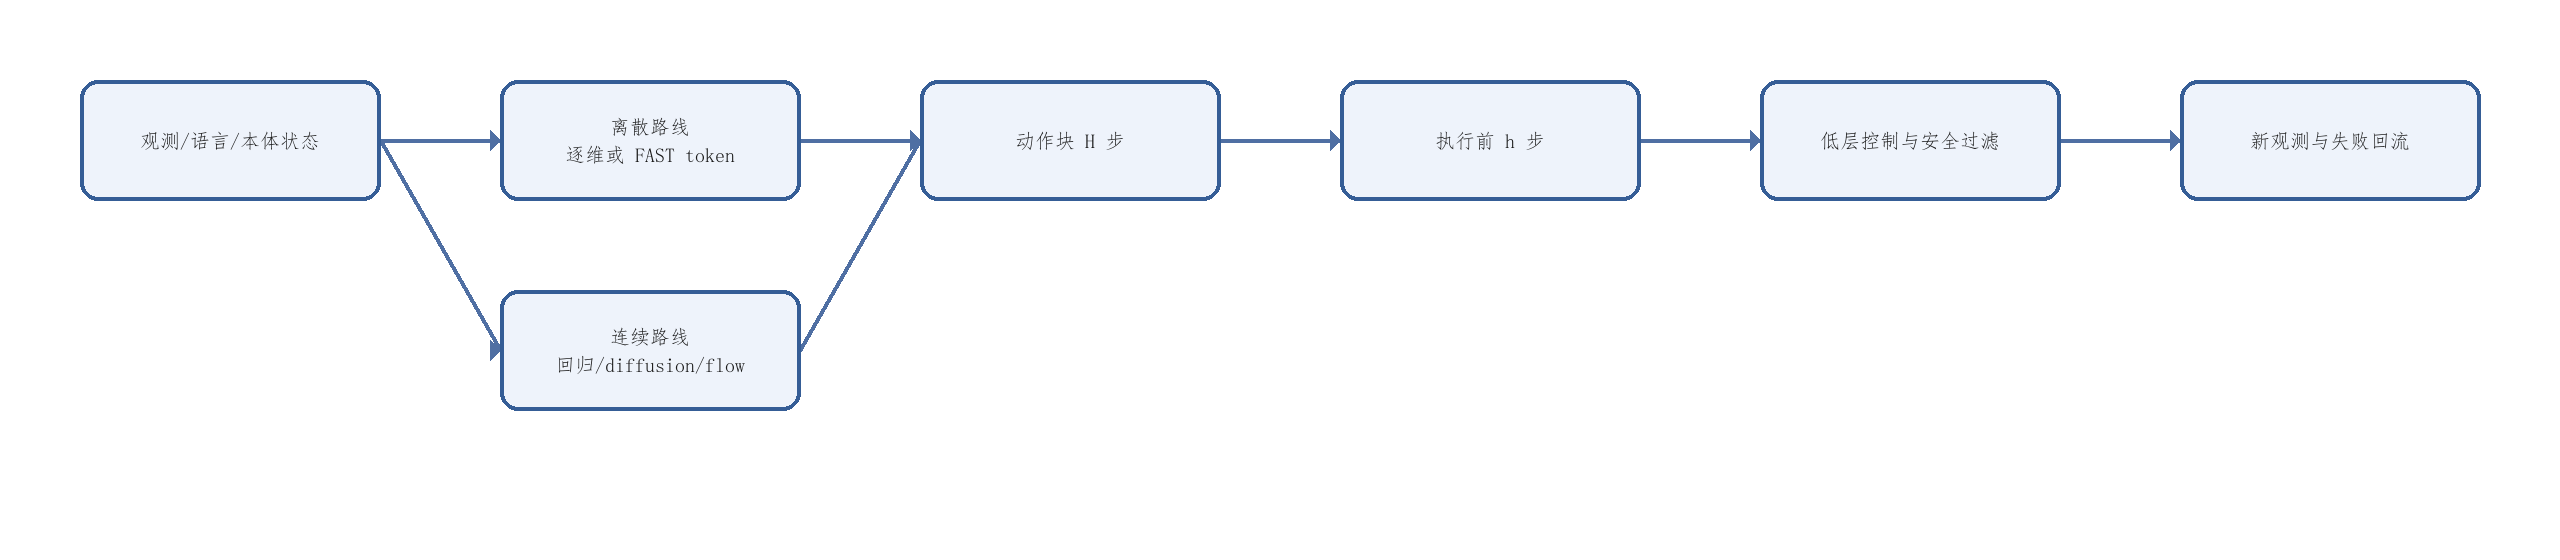
\includegraphics[width=\textwidth]{v0.3-23-VLA动作表示坐标.png}
\caption{动作表示、动作块与低层闭环之间的关系。作者依据 RT-2、Diffusion Policy、FAST 与 $\pi_0$ 的公开方法改绘\cite{brohan2023rt2,chi2023diffusion,pertsch2025fast,black2024pi0}。}
\label{fig:vla-action-design-space}
\end{figure}

\subsection{逐维回归：快，但容易把多峰行为平均掉}

若策略输出高斯均值，常用目标为
\begin{equation}
\mathcal L_{\mathrm{MSE}}=\mathbb E\|a_t-f_\theta(o_t,s_t,l)\|_2^2.
\end{equation}
它只需一次前向传播，适合低延迟控制；但当绕障可以向左也可以向右、抓取存在多个等价姿态时，条件均值可能落在两种可行动作之间。Mixture Density、离散 latent 或生成式动作头的目的，不是“让模型更大”，而是恢复条件动作分布的多峰结构。

这个结论可以直接从损失函数得到。对固定条件 $c=(o_t,s_t,l)$，把标量输出记为 $y$，则
\begin{equation}
\frac{\partial}{\partial y}\,\mathbb E[(a-y)^2\mid c]
=2\left(y-\mathbb E[a\mid c]\right),
\end{equation}
所以平方误差的最优点估计必为条件均值 $y^*=\mathbb E[a\mid c]$。若演示者以相同概率选择 $a=-1$ 和 $a=+1$，两种动作都可行，回归器却会输出 $0$。在绕障任务中，$0$ 可能恰好指向障碍物；这不是训练不足，而是“单峰点估计”与“多峰决策”之间的结构冲突。

\begin{figure}[H]
\centering
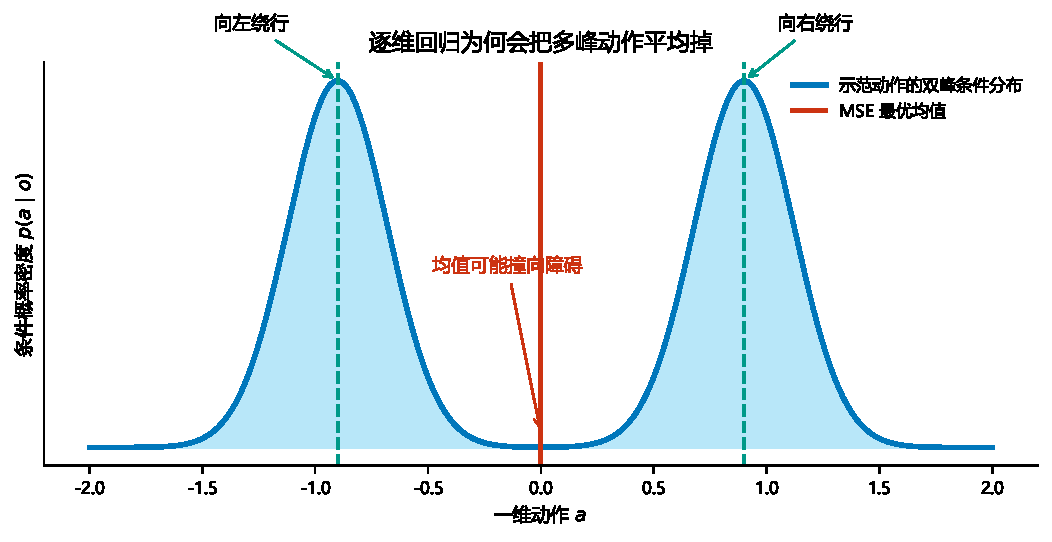
\includegraphics[width=0.92\textwidth]{v0.3-23-回归多峰平均.pdf}
\caption{平方误差把双峰动作分布压成条件均值的教学示意。曲线为作者生成的合成分布，不是论文实验结果。}
\label{fig:regression-mode-averaging}
\end{figure}

\subsection{离散动作 token：复用语言模型目标，但量化不是免费的}

将归一化动作 $a^{(j)}\in[-1,1]$ 均匀量化为 $B$ 个区间，
\begin{equation}
z^{(j)}=\operatorname{clip}\!\left(\left\lfloor\frac{a^{(j)}+1}{2}B\right\rfloor,0,B-1\right),
\qquad
\hat a^{(j)}=-1+\frac{2z^{(j)}+1}{B}.
\label{eq:uniform-action-token}
\end{equation}
于是训练可复用自回归交叉熵。RT-1 采用离散动作 token；RT-2 和 OpenVLA 让动作 token 与语言 token 共处输出词表\cite{brohan2022rt1,brohan2023rt2,kim2024openvla}。优势是训练基础设施成熟、输出概率可解释；代价是每个维度/时刻都占 token，量化误差与序列长度随控制维度和频率上升。

令分箱宽度 $\Delta=2/B$。若用箱中心解码且动作未被裁剪，单维最大量化误差为 $\Delta/2=1/B$；$B=256$ 时归一化误差上界约为 $0.0039$。这个数字必须乘回各维物理量程：同一归一化误差，对 $\pm1$ rad 的关节角与 $\pm0.1$ m 的位移不是同一控制误差。动作块含 $H$ 个时刻、每时刻有 $D$ 个独立离散维度时，朴素自回归序列长为 $DH$；例如 $D=7,H=50$ 就是 350 个动作 token。量化精度、解码延迟和上下文占用因此构成三方权衡。

\begin{figure}[H]
\centering
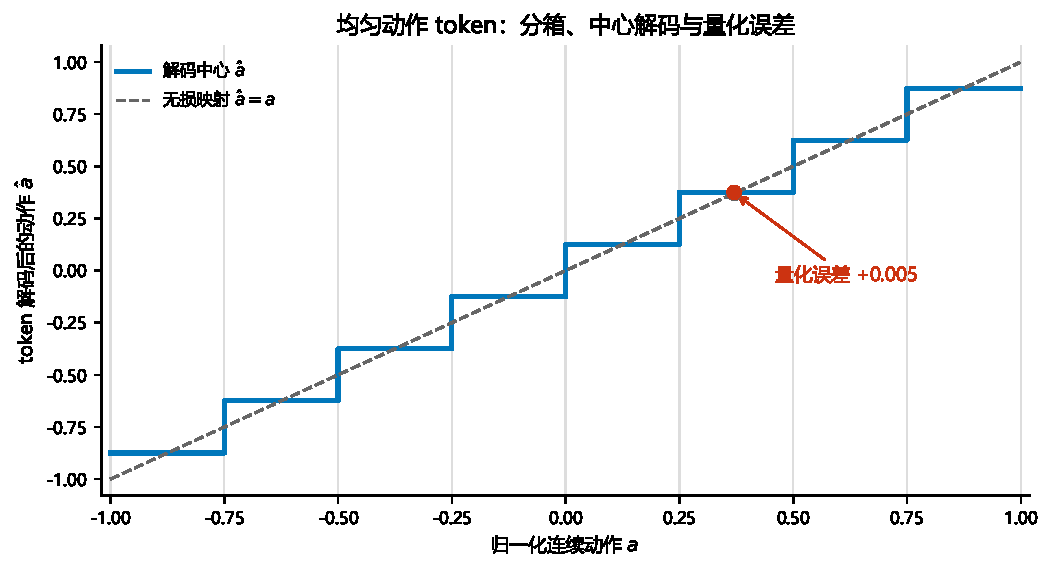
\includegraphics[width=0.94\textwidth]{v0.3-23-动作token量化.pdf}
\caption{均匀动作分箱的阶梯解码与误差。作者依据 OpenVLA 的动作 tokenizer 逻辑绘制\cite{kim2024openvla,openvla2024code}；图中使用 $B=8$ 仅为放大展示量化效应。}
\label{fig:action-token-quantization}
\end{figure}

FAST 指出逐维逐时刻分箱在高频灵巧动作上表现不佳，因而先对动作块做离散余弦变换，再对频域系数编码；FAST+ 在多机器人动作轨迹上学习通用 tokenizer\cite{pertsch2025fast}。这揭示了一个更一般的原则：动作 tokenizer 应利用时间相关性，而不是把每个采样点当作相互独立的“词”。

\subsection{扩散动作：表达多峰分布，以迭代换取计算}

令 $A^0=a_{t:t+H-1}$ 为干净动作块，前向过程加噪得到
\begin{equation}
A^\tau=\sqrt{\bar\alpha_\tau}A^0+\sqrt{1-\bar\alpha_\tau}\epsilon,
\qquad \epsilon\sim\mathcal N(0,I),
\end{equation}
噪声预测目标为
\begin{equation}
\mathcal L_{\mathrm{diff}}=
\mathbb E_{A^0,\tau,\epsilon}
\left\|\epsilon-\epsilon_\theta(A^\tau,\tau,o,s,l)\right\|_2^2.
\label{eq:diffusion-loss}
\end{equation}
推理从高斯噪声开始迭代去噪。Diffusion Policy 把这一过程与视觉条件、时间序列动作块和滚动时域执行结合，在其 12 项任务/4 组 benchmark 的实验集合中报告相对既有方法平均提升 46.9\%\cite{chi2023diffusion}。该数值不能直接与 OpenVLA 或 Gemini Robotics 的不同任务成功率相减。

训练和推理方向不能混为一谈。训练时先从数据集取干净动作 $A^0$，随机采样噪声等级 $\tau$ 和高斯噪声 $\epsilon$，只需构造一个带噪样本并回归噪声；推理时没有 $A^0$，必须从随机噪声出发，按噪声日程多次调用网络。不同随机初值可以收敛到不同动作模式，因此它能保留图\ref{fig:regression-mode-averaging}中被均值回归抹掉的选择。Diffusion Policy 还采用滚动时域：预测一段、执行前若干步、再用新观测重算；原论文 Fig.~3 把这件事与视觉条件去噪网络并列呈现\cite{chi2023diffusion}。

\begin{figure}[H]
\centering
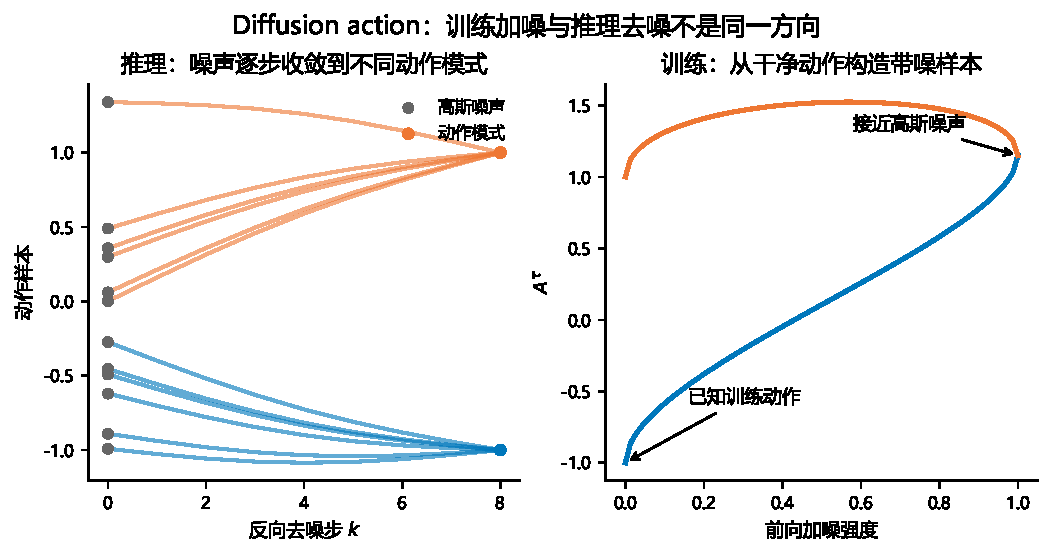
\includegraphics[width=\textwidth]{v0.3-23-扩散动作生成.pdf}
\caption{扩散动作的训练加噪与推理去噪方向。作者根据 Diffusion Policy 的方法与原论文 Fig.~1、Fig.~3 重新组织绘制\cite{chi2023diffusion}，不复制原图像素；轨迹为教学示意。}
\label{fig:diffusion-action-generation}
\end{figure}

Octo 采用 Transformer 主干和 diffusion readout，重点不是单一动作空间上的最高分，而是让不同相机、本体状态、任务条件和动作头以模块化 token group 接入，并在目标域小数据上微调\cite{octo2024}。扩散的工程代价是一次动作块需要多次网络评估；若动作块执行期间不重规划，快速生成并不等于快速闭环。

\subsection{流匹配：学习速度场，仍需数值积分}

取噪声 $A^0\sim\mathcal N(0,I)$、数据动作 $A^1\sim p_{data}$，线性概率路径
\begin{equation}
A^\tau=(1-\tau)A^0+\tau A^1,\qquad
u_\tau=A^1-A^0.
\end{equation}
流匹配训练速度场 $v_\theta$：
\begin{equation}
\mathcal L_{\mathrm{FM}}=
\mathbb E\left\|v_\theta(A^\tau,\tau,o,s,l)-u_\tau\right\|_2^2.
\label{eq:ch23-flow-matching}
\end{equation}
推理时积分 $dA/d\tau=v_\theta(A,\tau,\cdot)$。$\pi_0$ 在预训练 VLM 上接入 flow-matching 动作专家，以连续动作块覆盖单臂、双臂和移动操作平台\cite{black2024pi0}。与扩散相比，流匹配可使用较直接的常微分方程路径，但延迟仍取决于积分步数、主干缓存和硬件，不能由“flow”一词推断为单步控制。

具体地，以 $N$ 步显式 Euler 积分为例，$\Delta\tau=1/N$，
\begin{equation}
A_{i+1}=A_i+\Delta\tau\,v_\theta(A_i,\tau_i,o,s,l),
\qquad i=0,\ldots,N-1.
\label{eq:flow-euler}
\end{equation}
每一步都要在当前动作状态重新估计速度。$\pi_0$ 的公开论文实现以 PaliGemma 视觉语言主干配合约 300M 参数的动作专家，预测 $H=50$ 的动作块，并在所述实验中以 10 个 Euler 步完成积分\cite{black2024pi0}。其块状因果注意力允许视觉语言前缀被缓存，动作专家则在不同积分步更新；因此“10 步”不等于把整个大主干完整运行 10 次，但也绝不是一次前向传播。

\begin{figure}[H]
\centering
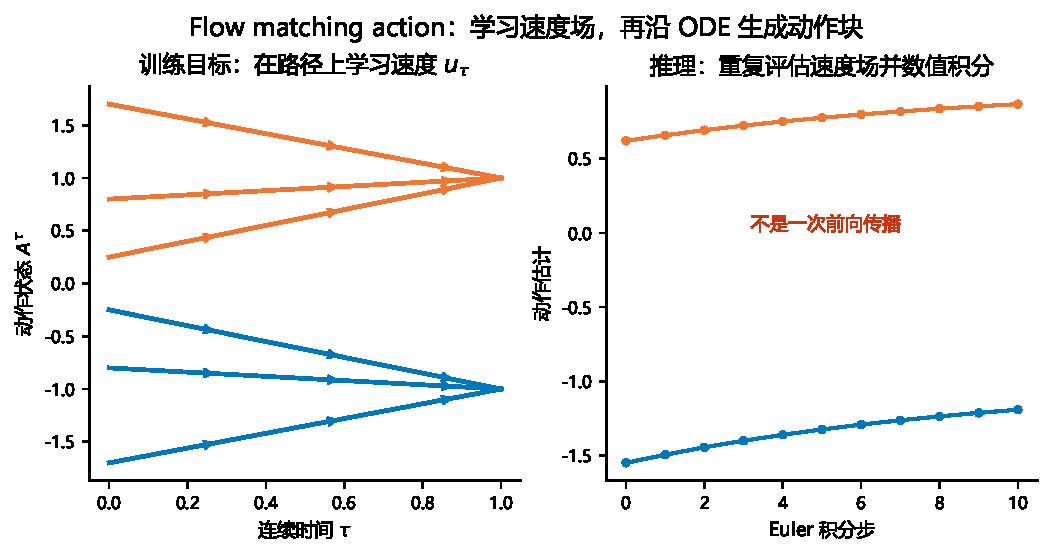
\includegraphics[width=\textwidth]{v0.3-23-流匹配动作生成.pdf}
\caption{流匹配的训练速度场与 Euler 推理。作者依据 $\pi_0$ 的 flow-matching 动作专家改绘\cite{black2024pi0}；路径为二维教学投影。}
\label{fig:flow-matching-action-generation}
\end{figure}

\section{动作块与闭环：$H$ 大不等于长时程智能}

预测 $H$ 步动作块能减少视觉主干调用并让动作在时间上连贯。部署时通常只执行前 $h\le H$ 步，再用新观测重规划。$h=H$ 接近开环动作块，延迟低但对扰动迟钝；$h=1$ 闭环最紧，但计算和通信压力最大。合理选择依赖三个时间尺度：相机/状态更新频率、VLA 推理时间和低层控制周期。

例如 50 Hz 动作数据、$H=50$ 表示 1 秒动作块。若模型用 200 ms 生成一次并执行前 10 步，则重规划周期为 200 ms；若执行全部 50 步，模型虽能提前 800 ms 空闲，却可能在物体被移动后继续执行旧动作。论文若只写“输出 50-step chunk”而不报告 $h$、推理延迟、低层跟踪和观测新鲜度，读者无法判断闭环能力。

\section{主干与动作头如何分工}

PaLM-E 把图像、连续状态估计和文本编码交错输入语言模型，证明具身传感可以进入大型多模态主干，但其代表性机器人任务更多落在具身推理和规划，并不等价于一个高频低层控制策略\cite{driess2023palme}。RT-2 则明确把动作写入 VLM 输出空间，使网页语义预训练与机器人控制共同训练\cite{brohan2023rt2}。这一区分阻止了常见误写：不能因为模型“看见机器人并输出计划”就把它归为直接动作 VLA。

RT-1 的输入端以 EfficientNet 提取图像特征，并用 FiLM 接入语言条件；TokenLearner 压缩视觉 token 后，Transformer 按时间建模并输出离散动作。RT-2 改变的关键并非“再加一层 Transformer”，而是把机器人动作写进 VLM 的文本化输出空间，以网页视觉语言任务与机器人轨迹共同训练。PaLM-E 则把连续传感编码成与文本 token 同维的嵌入插入语言模型，更适合作为“感知信息如何进入具身推理主干”的代表。三者都使用 Transformer，但输入组织、监督目标和控制责任不同。

OpenVLA 组合 DINOv2 与 SigLIP 视觉特征、Llama 2 语言主干和离散动作输出，在 970k 真实机器人示范上训练；论文报告其 7B 模型在指定 29 项任务设置中相对 RT-2-X 的绝对成功率优势，以及相对从头训练 Diffusion Policy 的目标域微调优势\cite{kim2024openvla}。这些结果支持其设计在该评测协议下有效，不支持“7B 普遍优于 55B”这种脱离数据与动作接口的结论。

OpenVLA 中，DINOv2 偏向局部视觉表征，SigLIP 提供视觉--语言对齐特征，两路特征拼接后经投影器送入 Llama 2；动作再由语言模型词表末端的一组 token 自回归产生。于是视觉编码器回答“看到了什么”，投影器解决维度/分布接口，语言主干融合指令与图像上下文，ActionTokenizer 才负责连续控制量的编解码。任何一层冻结或微调，都会改变数据需求与部署代价，不能用“Llama 2 输出动作”一句话概括。

图\ref{fig:openvla-original-architecture}给出原论文的完整接口关系。读图时应沿编号 $1\rightarrow2\rightarrow3$ 追踪：DINOv2 与 SigLIP 分别编码同一图像，特征经 MLP projector 投到语言嵌入空间，再与指令 token 一起进入 Llama 2；输出端的 action de-tokenizer 才把词表 token 还原成七维控制量。原图把“视觉融合”和“动作反量化”画在主干两端，说明 OpenVLA 不是把连续向量直接塞给语言模型，而是依赖两个机器人专用接口夹住通用 VLM 主干。

\begin{figure}[H]
\centering
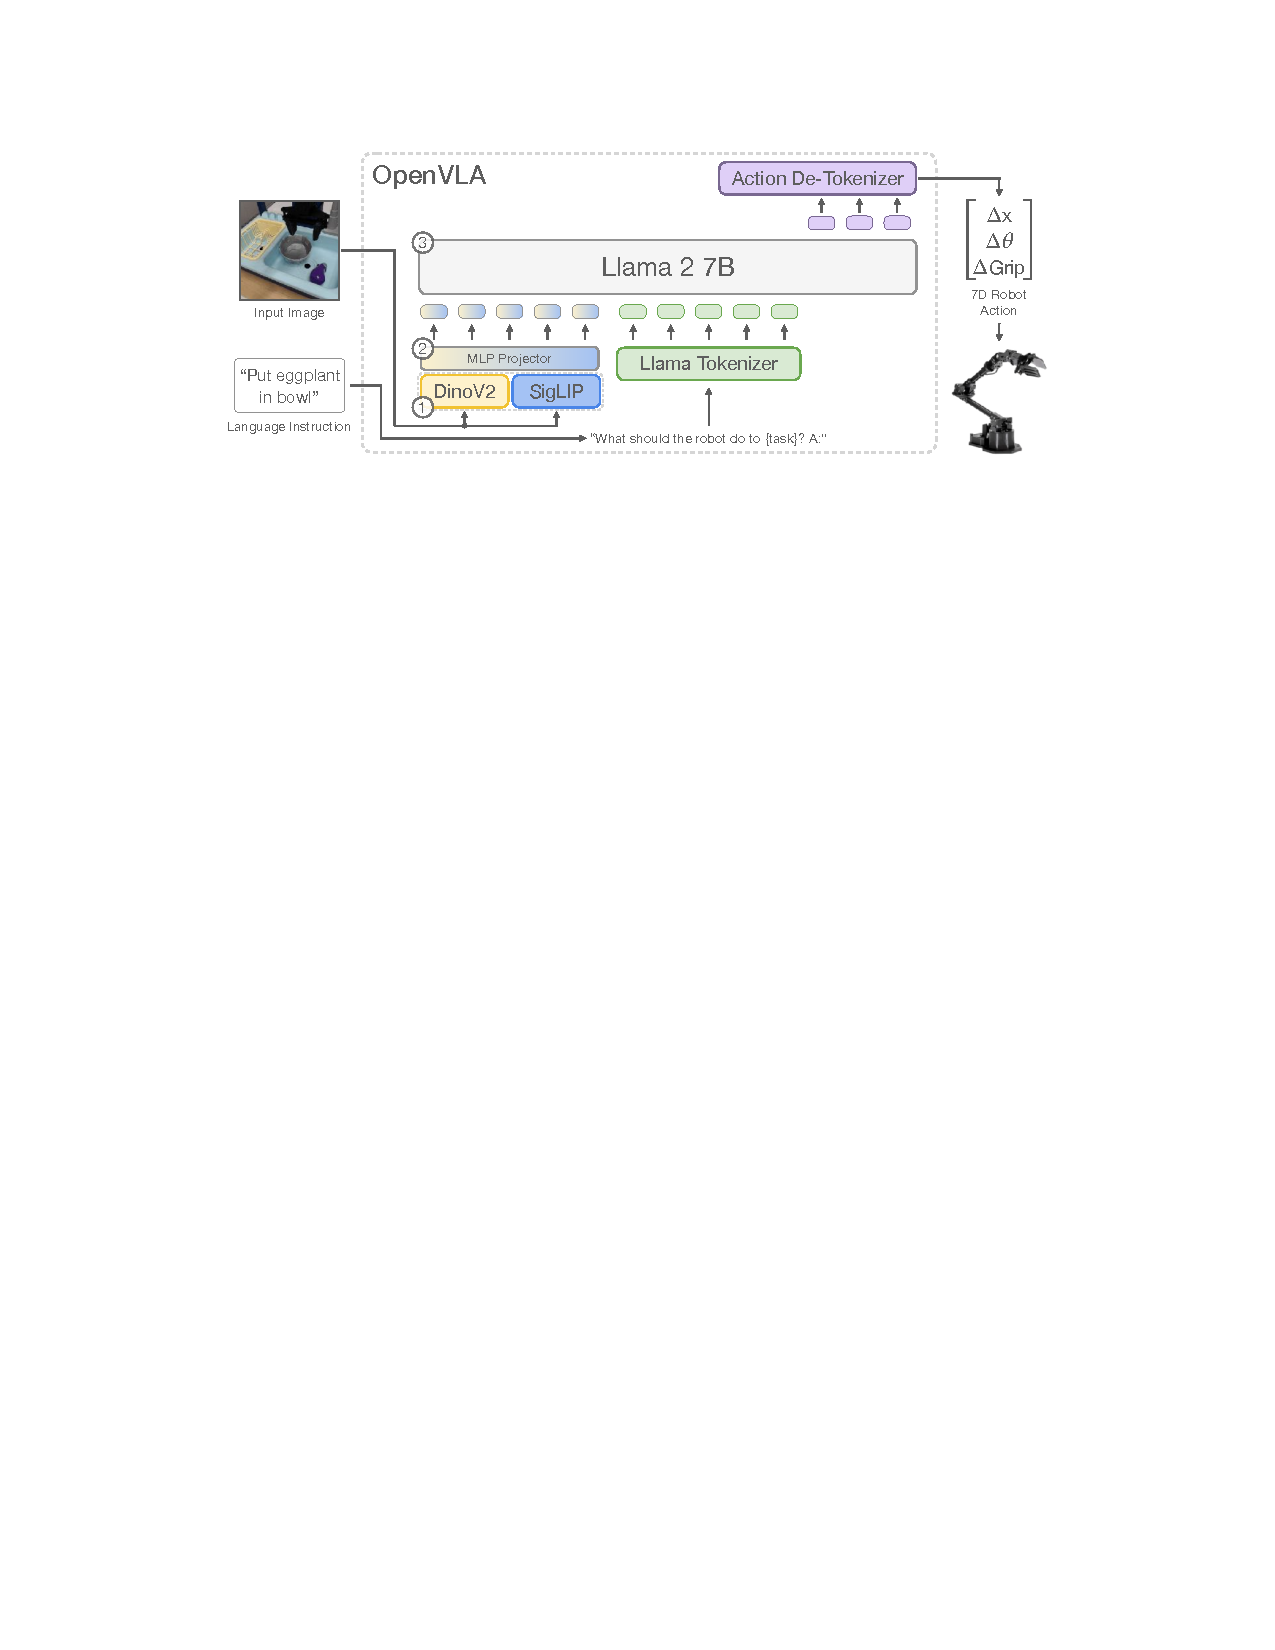
\includegraphics[width=0.96\textwidth]{v0.3-23-OpenVLA-Fig2原图.pdf}
\caption{OpenVLA 模型架构原图。引自 OpenVLA 原论文 Fig.~2（arXiv:2406.09246v3）\cite{kim2024openvla}，CC BY 4.0；从论文第 4 页裁切，仅缩放，未翻译或改绘。}
\label{fig:openvla-original-architecture}
\end{figure}

\subsection{Octo：模块化不是一句“可扩展”}

Octo 的主干输入由若干 \emph{token group} 组成：任务侧可以是语言或目标图像，观测侧可以包含多相机图像和本体状态。各自 tokenizer 先把异构输入变成统一宽度的 token，再由块状注意力掩码规定哪些组能相互读取。主干不直接把最后一个普通 token 当动作，而是加入专用 readout token；readout 汇聚上下文后连接 diffusion action head，产生连续动作块\cite{octo2024}。

这种设计把“共享知识”和“本体接口”分开。迁移到新机器人时，可以增加新的观测 tokenizer 以接收力/力矩或不同相机，也可以替换动作 readout 以适配新的关节维度；共享 Transformer 仍提供从 25 个数据集、约 80 万段轨迹中学到的跨任务表征。它并不意味着零成本跨本体：新增模块仍需目标域数据训练，动作归一化、时间对齐和相机标定也必须重做。

原论文 Fig.~2 还表达了改绘图容易弱化的一点：预训练序列可以反复交错 observation 与 readout，而微调阶段以虚线模块加入新观测和新动作空间。图\ref{fig:octo-original-architecture}保留这一原始视觉编码；图\ref{fig:octo-modular-architecture}则将其重排成中文模块图，便于逐步解释 tokenizer、主干、readout 和动作头的职责。两图承担不同任务，不作为重复插图计数。

\begin{figure}[H]
\centering
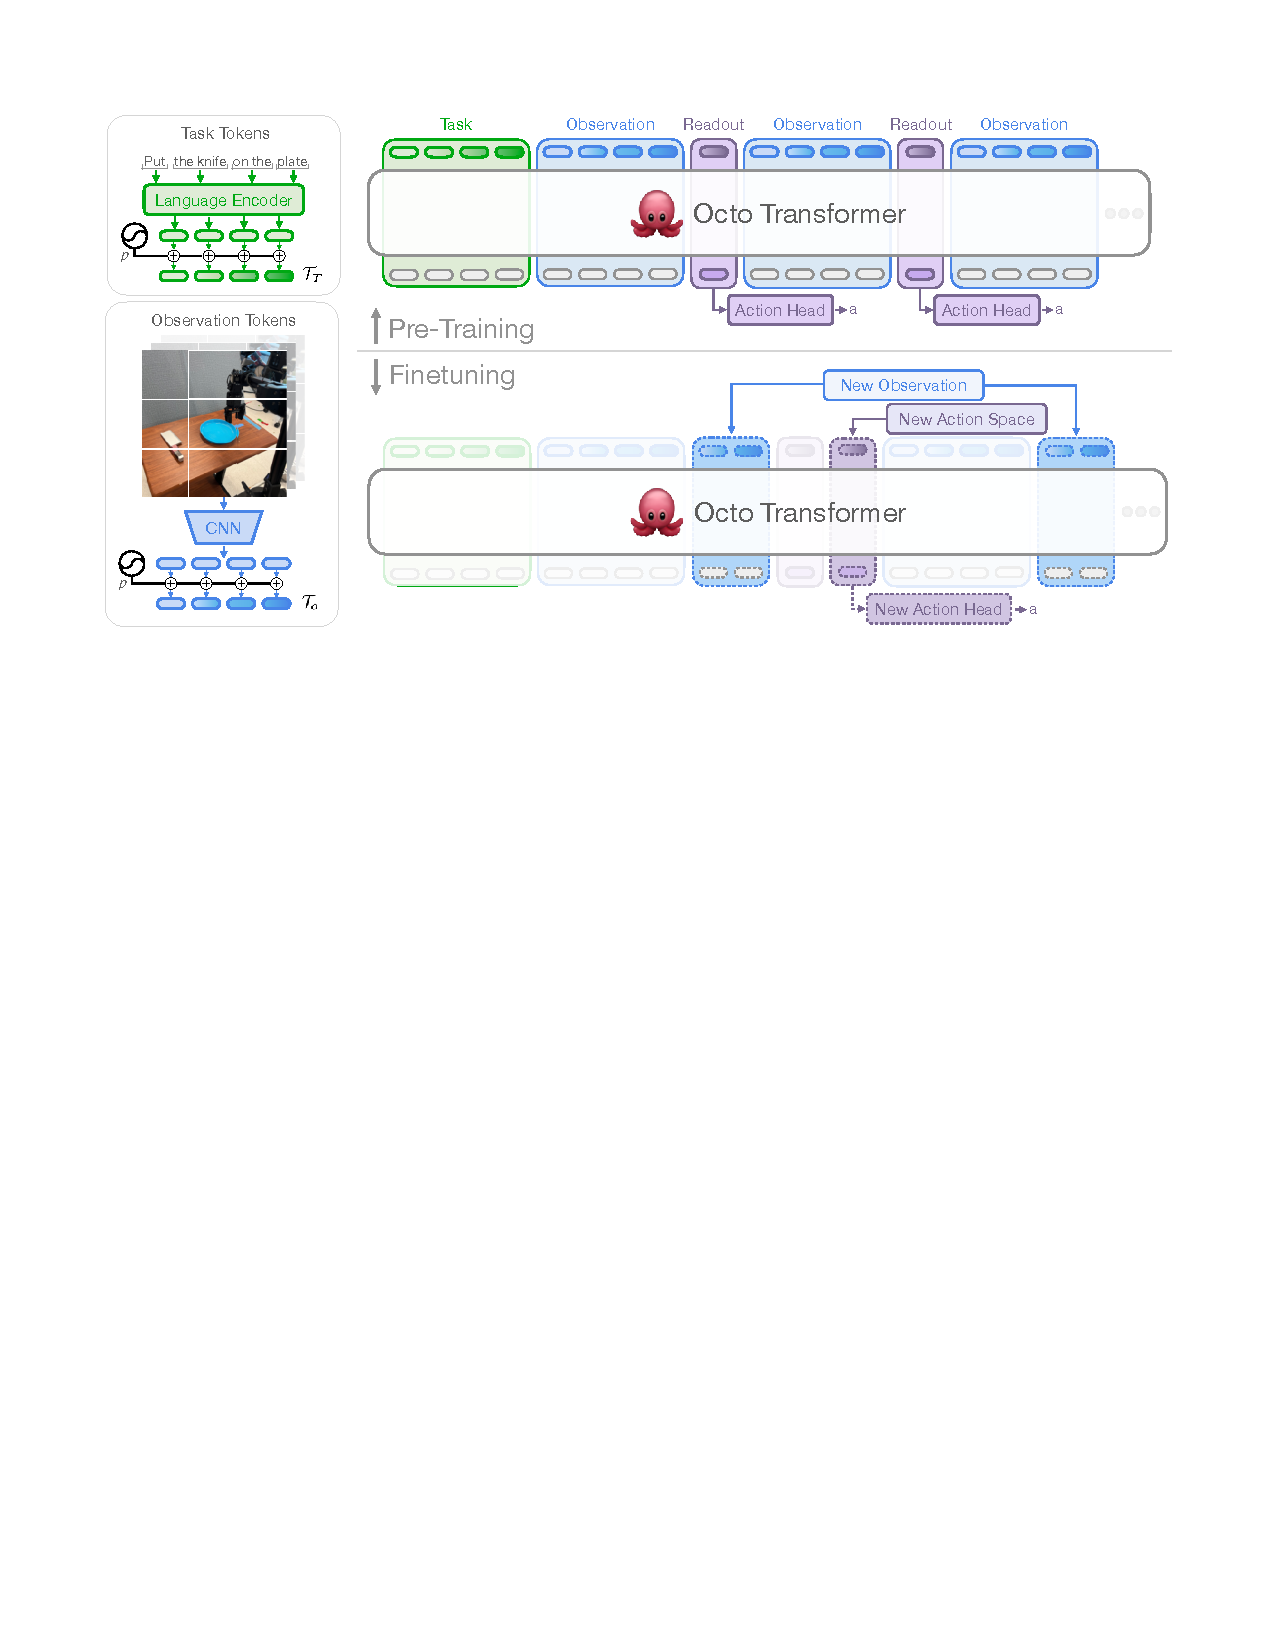
\includegraphics[width=\textwidth]{v0.3-23-Octo-Fig2原图.pdf}
\caption{Octo 模型架构原图。引自 Octo 原论文 Fig.~2（arXiv:2405.12213v2）\cite{octo2024}，CC BY 4.0；从论文第 3 页裁切，仅缩放，未翻译或改绘。}
\label{fig:octo-original-architecture}
\end{figure}
\endgroup

\begin{figure}[H]
\centering
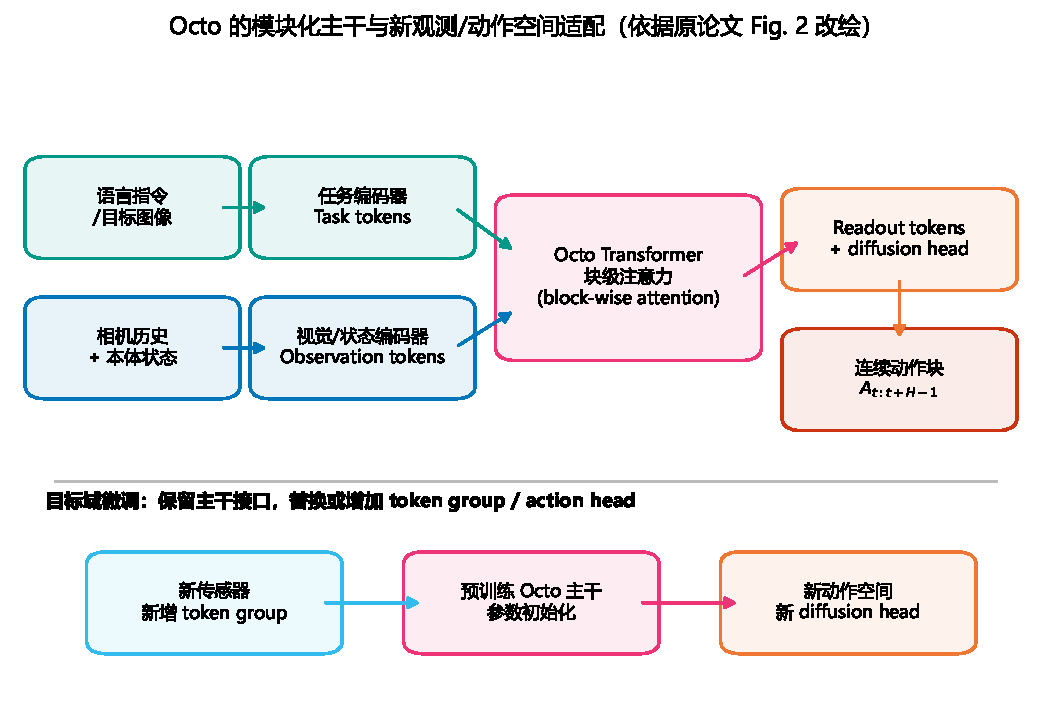
\includegraphics[width=\textwidth]{v0.3-23-Octo模块化架构.pdf}
\caption{Octo 的模块化输入、Transformer 主干、readout 与动作头，以及目标域新增接口。作者依据 Octo 原论文 Fig.~2 改绘\cite{octo2024}，不复制原图像素。}
\label{fig:octo-modular-architecture}
\end{figure}

GR00T N1 把 VLM System 2 与 diffusion transformer System 1 紧耦合并端到端训练，数据混合真实轨迹、人类视频和合成样本\cite{nvidia2025groot}。Gemini Robotics 报告直接控制 VLA；同一技术报告另设 Gemini Robotics-ER，负责空间/时间理解、指向、轨迹与抓取预测等具身推理能力\cite{gemini2025robotics}。二者都提供重要系统证据，但完整训练代码、数据和权重并未公开到足以复现论文主张的程度，开源程度必须与论文新颖性分开评价。

\begingroup
\hbadness=10000
\begin{table}[H]
\centering
\caption{代表性路线的统一设计比较；结果数值因任务与协议不同，不作横向排行榜}
\label{tab:vla-design}
\scriptsize
\begin{tabularx}{\textwidth}{p{0.105\textwidth}p{0.14\textwidth}p{0.13\textwidth}p{0.13\textwidth}p{0.14\textwidth}Y}
\toprule
路线 & 主干/融合 & 动作表示 & 时序与闭环 & 开放证据 & 主要适用条件与限制\\
\midrule
RT-1 & EfficientNet/\allowbreak FiLM、TokenLearner、Transformer & 逐维离散 token & 短历史、实时逐步策略 & 论文与部分官方代码 & 单平台大规模多任务；语义主干不来自通用 VLM\\
PaLM-E & 传感编码与文本 token 交错进 LLM & 以语言/规划输出为主 & 高层推理接口 & 论文，模型闭源 & 不能直接当作低层 VLA 基线\\
RT-2 & VLM 与机器人数据共同训练 & 动作作为文本 token & VLA 直接控制 & 论文，主模型闭源 & 语义迁移强；量化、解码与闭环细节受实现约束\\
Diffusion Policy & 视觉编码器+条件去噪网络 & 连续 diffusion chunk & receding horizon & 论文和官方代码 & 多峰连续动作；多步去噪增加延迟\\
Octo & 模块化 Transformer & diffusion readout & chunk+目标域微调 & 论文、权重、代码 & 新观测/动作空间适配；规模小于大 VLM 路线\\
OpenVLA & DINOv2+\allowbreak SigLIP+\allowbreak Llama 2 & 256-bin 离散 token & 自回归动作输出 & 论文、权重、MIT 代码 & 易复用语言模型栈；高频动作 token 长度和量化受限\\
$\pi_0$ & 预训练 VLM+动作专家 & flow-matching chunk & 数值积分后滚动执行 & 论文、部分权重与 Apache-2.0 代码 & 灵巧连续动作；推理步数和跨本体适配仍需工程验证\\
GR00T N1 & VLM System 2 + DiT System 1 & diffusion action & 双系统端到端 & 报告与开放模型范围 & 人形双臂；开放资产与论文全训练栈并非完全等价\\
Gemini Robotics & Gemini 2.0 基础与机器人专用后训练 & 报告为直接连续控制 & 强调反应式闭环 & 技术报告，核心闭源 & 能力覆盖广；第三方复现与接口细节有限\\
\bottomrule
\end{tabularx}
\end{table}
\endgroup

\section{真实源码导读：OpenVLA 的均匀动作分箱}

OpenVLA 的 \texttt{ActionTokenizer} 清楚展示了式\eqref{eq:uniform-action-token}如何进入代码：先裁剪到动作范围，再逐维分箱，并把分箱编号映射到词表尾部的低频 token\cite{openvla2024code}。

\begin{lstlisting}[language=Python,caption={OpenVLA ActionTokenizer 的关键路径（MIT；为节省篇幅删去类型与批处理分支）}]
self.bins = np.linspace(min_action, max_action, self.n_bins)
self.bin_centers = (self.bins[:-1] + self.bins[1:]) / 2.0

action = np.clip(action, a_min=float(self.min_action),
                 a_max=float(self.max_action))
discretized_action = np.digitize(action, self.bins)
token_ids = self.tokenizer.vocab_size - discretized_action

discretized = self.tokenizer.vocab_size - action_token_ids
discretized = np.clip(discretized - 1, 0,
                      self.bin_centers.shape[0] - 1)
actions = self.bin_centers[discretized]
\end{lstlisting}
\sourceanchor{仓库 \path{openvla/openvla}；许可证 MIT；commit \texttt{c8f03f48\allowbreak af692657\allowbreak d3060c19\allowbreak 588038c7\allowbreak 220e9af9}；文件 \path{prismatic/vla/action_tokenizer.py}；符号 \texttt{ActionTokenizer}。代码逻辑已按 2026-07-13 的 \texttt{main} 页面核验；2026-07-14 通过只读远端查询固定当日 \texttt{main} HEAD，并使用 immutable permalink。}

代码暴露了三个模型图中不易看见的假设。第一，所有动作维统一裁剪到 $[-1,1]$，因此数据统计和反归一化是控制接口的一部分。第二，分箱边界有 256 个而中心只有 255 个，解码需要边界裁剪；“256 个 action token”不等于 256 个等宽可还原中心。第三，映射占用基础 tokenizer 词表末端 token，动作与语言共享词表是工程约定，不是物理上自然的表示。

\section{如何读实验表：先校准任务，再看数字}

跨论文比较至少检查五项：训练数据是否包含测试机器人；任务是 zero-shot、目标域微调还是从头训练；成功判据和试验次数；动作空间与控制频率；是否允许人工复位、重试或高层规划器。Octo 的官方评测覆盖 9 个真机 setup，并报告新力/力矩观测和新关节动作空间的微调\cite{octo2024}；OpenVLA 的 29 项任务、RT-1 的 700+ 数据采集任务与 Gemini Robotics 的能力演示不是同一统计总体。

因此本章不制作“综合成功率排名”。可以比较的是同一论文内部的受控消融，例如 OpenVLA 的视觉特征组合、Octo 的数据/架构选择、Diffusion Policy 的滚动执行与时间序列设计；跨论文只能比较证据边界和接口属性。对闭源模型，作者视频可以证明某次演示发生过，却不能估计总体成功率或失败分布。

\section{知识小结与综述判断}

\textbf{知识小结。}离散 token 把连续动作转成语言模型可处理的分类目标，但引入量化与序列长度；扩散和流匹配能表达多峰连续动作，却需要迭代去噪或数值积分；action chunk 在时间一致性、推理摊销和闭环反应之间权衡。主干是否具备视觉语言知识、动作头是否承担低层控制、执行后何时重规划，是比模型参数量更有解释力的坐标。

\authorjudgement{VLA 研究的核心竞争并不是“谁把最大的 VLM 接到机器人上”，而是谁能在语义泛化、动作分布表达、闭环频率、跨本体归一化和可复现评测之间形成可部署的组合。当前证据尚不足以宣告离散 token、diffusion 或 flow matching 中任何一种取得普遍胜利。对接触密集任务，VLA 最合理的输出通常是受约束动作块或技能参数，仍由本书动力学与接触章定义的实时控制、安全限幅和恢复状态机执行。}

\chapter[VLA 数据、训练目标、评测与泛化]{VLA 数据、训练目标、\\评测与泛化}
\label{chap:vla-data-evaluation}

\section{多机器人数据的难点是语义对齐，不是文件拼接}

Open X-Embodiment 把多机构机器人数据组织为标准格式，并用 RT-X 探索跨机器人正迁移\cite{openx2024}。标准 schema 解决“字段放在哪里”，却不自动解决动作语义：末端增量的参考坐标、夹爪正负方向、控制周期、相机命名和成功标签仍可能不同。每个 episode 至少需要机器人 ID、任务语言、观测/动作 schema 版本、坐标约定、标定、时间戳、终止原因和来源许可证。

设数据集 $D_i$ 有 $N_i$ 个 episode，训练采样权重为 $w_i$，则模型实际优化的是
\begin{equation}
\mathcal L=\sum_i w_i\,\mathbb E_{\tau\sim D_i}
\left[\sum_t m_{i,t}\ell_\theta(\tau_t)\right],\qquad \sum_iw_i=1,
\label{eq:vla-mixture-loss}
\end{equation}
其中 $m_{i,t}$ 是有效动作维/时间掩码。若令 $w_i=N_i/\sum_jN_j$，最大数据源会主导；若数据集等权，小型噪声集会被过采样。Octo 的多数据集训练\cite{octo2024}和 OpenVLA 的大规模真实示范训练\cite{kim2024openvla}都必须连同混合权重与规范化解释。

\begin{table}[H]
\centering
\caption{跨机器人数据混合的对齐检查}
\label{tab:vla-data-alignment}
\begin{tabularx}{\textwidth}{p{0.16\textwidth}YYYY}
\toprule
字段 & 必须记录 & 可统一内容 & 不应强行统一 & 错配后果 \\
\midrule
动作 & 坐标、单位、频率、维数 & 通用目标 schema & 关节拓扑与执行器限制 & 方向反转、尺度失控 \\
图像 & 相机 ID、时间、内外参 & 张量布局、颜色空间 & 视角与遮挡分布 & 错把相机差异当任务差异 \\
语言 & 原文、重写来源、任务 ID & tokenizer 接口 & 粒度与歧义 & 重复措辞支配任务采样 \\
终止 & 成功/失败/截断原因 & 枚举字段 & 场景特定判据 & 截断被误作成功或负例 \\
\bottomrule
\end{tabularx}
\end{table}

\section{归一化是模型接口的一部分}

对动作维 $j$，常用分位数归一化
\begin{equation}
\tilde a_j=2\frac{\operatorname{clip}(a_j,q_j^- ,q_j^+)-q_j^-}
{q_j^+-q_j^-}-1.
\end{equation}
$q_j^\pm$ 必须与机器人、动作 schema 和训练版本绑定。若部署时使用另一数据集统计量，张量形状仍正确，却会系统改变速度或位移。离散 token 又在归一化之后分箱，因此错误会被合法 token 掩盖。第 23 章的 OpenVLA 源码导读展示了这一边界。

\section{目标函数：共享主干不代表监督等价}

动作行为克隆可与语言生成、图文对比、价值或成功预测联合：
\begin{equation}
\mathcal L_{\mathrm{total}}=\lambda_a\mathcal L_{\mathrm{act}}
+\lambda_l\mathcal L_{\mathrm{lang}}+\lambda_v\mathcal L_{\mathrm{vision}}
+\lambda_s\mathcal L_{\mathrm{success}}.
\end{equation}
辅助目标能保留语义或改善表征，但也可能占用容量并与精细控制冲突。RT-2 通过视觉语言与机器人数据共训练研究知识迁移\cite{brohan2023rt2}；这类结论应由动作任务消融支持，而不能从 VLM 指标直接外推。

后训练还包括目标域微调、低秩适配、失败数据回放和偏好/价值校正。比较时必须标明：基础模型是否相同、目标域示范数、哪些层更新、是否使用评测环境数据、是否按最佳 checkpoint 选择。否则“少样本适配”可能隐含大量预训练覆盖或测试集调参。

\section{把“泛化”拆成四个正交问题}

任务泛化是新指令/技能组合；对象泛化是新实例或类别；场景泛化是背景、布局、光照和干扰变化；本体泛化是新机器人几何、传感器与动作接口。四者可同时变化，但证据强度不同。若新对象出现在相同桌面、相同相机且动作相同，只能支持对象轴结论；不能写成“开放世界泛化”。

\begin{table}[H]
\centering
\caption{VLA 评测证据的可比性边界}
\label{tab:vla-evidence-comparability}
\begin{tabularx}{\textwidth}{p{0.17\textwidth}YYYY}
\toprule
证据 & 可回答问题 & 必报条件 & 不能单独回答 & 常见误用 \\
\midrule
离线动作指标 & 数据拟合、量化/时延诊断 & 划分、掩码、归一化 & 闭环成功、安全 & 用 MSE 排名多峰策略 \\
仿真 & 大样本闭环比较 & 版本、种子、物理/视觉设置 & 真机可靠性 & 忽略 simulator gap \\
真机成功率 & 指定协议下任务结果 & 次数、初态、失败判据 & 广泛泛化 & 小样本百分比当稳定结论 \\
恢复/安全 & 扰动后的系统韧性 & 扰动、介入、风险定义 & 单模型能力 & 把安全层功劳归给 VLA \\
\bottomrule
\end{tabularx}
\end{table}

\section{成功率必须带不确定性}

若 $n$ 次试验成功 $k$ 次，点估计 $\hat p=k/n$。Wilson 区间为
\begin{equation}
\frac{\hat p+z^2/(2n)\pm z\sqrt{\hat p(1-\hat p)/n+z^2/(4n^2)}}
{1+z^2/n}.
\label{eq:wilson-success}
\end{equation}
例如 10 次成功 8 次并不等价于大样本下稳定的 80\%。论文若只给平均百分比、不报告试验次数、跨种子/任务方差和人工介入，就不能支持微小模型差异。

\begin{lstlisting}[caption={可复核真机评测协议的最小记录循环}]
for trial in preregistered_trials:
    reset_to_recorded_initial_state(trial.reset_id)
    start = capture_state_and_versions()
    result = run_with_fixed_timeout(policy, trial.instruction)
    outcome = independent_success_check(result, trial.success_rule)
    write_record(trial_id=trial.id, outcome=outcome,
                 intervention=result.human_interventions,
                 recovery=result.recovery_events,
                 safety=result.constraint_events,
                 model_hash=MODEL_HASH, start_state=start)
report_counts_and_confidence_intervals(group_by=["task", "generalization_axis"])
\end{lstlisting}

\section{怎样核查 SOTA 声明}

逐项检查任务是否相同、初态难度是否相同、是否允许重试/人工介入、控制频率和硬件是否相同、基线是否使用相同目标域数据、模型选择是否接触测试集。只要任一项不同，应写“在各自协议下报告”，而不是排序。第 23 章中的模型数字因此只支持论文指定设置的设计判断。

\section{知识小结与综述判断}

VLA 证据链从 schema 和动作语义开始，经采样权重、归一化、训练目标与后训练，最后落到分轴泛化和带置信区间的闭环评测。综述判断是：模型规模或平均成功率都不是独立证据；只有数据暴露、适配预算、试验协议与失败处理同时可比时，性能排序才有意义。

\chapter[开源复现、代码路径与部署接口]{开源复现、代码路径\\与部署接口}
\label{chap:vla-reproduction}

\section{复现对象：结果、训练还是部署}

“跑通仓库”至少有三种含义：用官方权重完成离线推理；在指定数据上重现微调趋势；接入真实机器人闭环。三者成本和证据强度递增。本章选择 OpenVLA 与 Octo 两条 MIT 开源路线，固定到 OpenVLA commit \texttt{c8f03f48...} 和 Octo release \texttt{v1.5}；不把网页当前 \texttt{main} 当可复现版本\cite{openvla2024code,octo15code}。

\begin{table}[H]
\centering
\caption{两条开源 VLA 路线的可复核执行链}
\label{tab:open-vla-repro-paths}
\begin{tabularx}{\textwidth}{p{0.14\textwidth}YYYY}
\toprule
路线 & 固定版本 & 模型/训练入口 & 动作接口 & 复现重点 \\
\midrule
OpenVLA & commit \texttt{c8f03f48...} & \path{vla-scripts/finetune.py}；Prismatic VLA & 离散 token 反量化为连续动作 & tokenizer、数据统计、VLM 显存 \\
Octo & release \texttt{v1.5} & \texttt{OctoModel}、模块化 transformer/readout & diffusion 动作采样 & task、mask、历史窗、动作统计 \\
\bottomrule
\end{tabularx}
\end{table}

第 23 章已逐行解释 OpenVLA \texttt{ActionTokenizer} 的均匀分箱，并记录完整 commit、文件与符号。这里不重复源码，而把它放回执行链：数据适配器计算动作统计，训练目标生成 action token，推理端反量化，机器人适配器再恢复真实单位与坐标。任何一步版本错配都会输出“合法但危险”的动作。

\section{环境与权重必须成为 manifest}

复现 manifest 至少包含代码 commit/tag、Python/CUDA/JAX/PyTorch 版本、锁文件哈希、权重 URL 与校验和、数据版本、GPU 型号、精度、随机种子和命令行。权重能加载不代表兼容：tokenizer 词表、视觉预处理或配置字段变化都可能不报错地改变结果。

\begin{lstlisting}[caption={建议的复现 manifest 骨架，不以浮动 latest 作为版本}]
experiment: octo_offline_smoke_test
repository: https://github.com/octo-models/octo
revision: v1.5
license: MIT
python: "3.10.x"
framework: "jax/flax versions from locked environment"
checkpoint: "octo-base-1.5"
checkpoint_sha256: "<record after verified download>"
dataset_schema: "oxe/rlds + local adapter v3"
robot_adapter: "widowx_delta_ee_v2"
action_statistics_hash: "<sha256>"
\end{lstlisting}

尖括号字段表示构建者必须在实际下载后填写，不能由报告编造。初稿的价值在于定义放行条件；最终冻结前应在目标机器生成真实 manifest 和日志。

\section{Octo：task、观测掩码与动作采样}

Octo 的官方入口把模型加载、任务创建和动作采样分开\cite{octo15code}。下列关键调用依据 \texttt{v1.5} README/API 压缩，保留决定接口的语句：

\begin{lstlisting}[language=Python,caption={Octo v1.5 推理关键路径（MIT；按官方 API 压缩）}]
model = OctoModel.load_pretrained("hf://rail-berkeley/octo-base-1.5")
task = model.create_tasks(texts=["pick up the red cup"])

observation = {
    "image_primary": image[None, None],
    "timestep_pad_mask": np.array([[True]]),
}
actions = model.sample_actions(
    observation, task,
    unnormalization_statistics=dataset_statistics["action"],
    rng=jax.random.PRNGKey(seed),
)
\end{lstlisting}
\sourceanchor{仓库 \path{octo-models/octo}；许可证 MIT；release \texttt{v1.5}；主要入口 \path{octo/model/octo_model.py} 的 \texttt{OctoModel.load\_pretrained}、\texttt{create\_tasks} 与 \texttt{sample\_actions}。本段依据官方 release README/API 压缩；未声明逐字复制某一连续行段。}

\texttt{timestep\_pad\_mask} 不是装饰字段：历史窗口开头缺帧时，它阻止填充值进入注意力。\texttt{unnormalization\_statistics} 决定动作恢复尺度。模型预训练动作块长度为 4 时，可以执行全部四步，也可以只执行首步滚动重规划；两种部署协议的时延和扰动恢复不同。

\section{OpenVLA：数据微调与动作 token 接口}

OpenVLA 把图像和指令送入 VLM 主干，再输出动作 token\cite{kim2024openvla}。复现路径应按顺序验证：官方权重单样本前向；tokenizer 编解码往返；目标数据 RLDS/schema 适配；小批过拟合；固定任务微调；离线回放；仿真或影子模式；低速真机。直接从“权重加载成功”跳到真机，会同时暴露图像通道、动作统计、坐标变换和控制周期错误。

一个重要单元测试是
\begin{equation}
\epsilon_{\mathrm{roundtrip}}=
\left\|\boldsymbol a-operatorname{decode}(\operatorname{encode}(\boldsymbol a))\right\|_\infty,
\end{equation}
并分别在分箱中心、边界、裁剪外值测试。该误差只能验证量化实现，不能证明机器人动作语义正确；还需用已知末端运动做坐标与单位测试。

\section{机器人适配层：把模型输出变成可拒绝的候选}

\begin{lstlisting}[caption={部署适配器的最小失败链}]
def deploy_vla(model, raw_observation, robot_contract):
    obs = robot_contract.preprocess_and_timestamp(raw_observation)
    assert obs.schema_hash == model.expected_schema_hash
    normalized_action = model.predict_action(obs)
    action = robot_contract.denormalize(normalized_action)
    command = robot_contract.to_control_frame(action)
    if not robot_contract.dimension_unit_and_rate_valid(command):
        return reject("adapter_contract_violation")
    if not shadow_mode_agrees_with_limits(command):
        return reject("shadow_validation_failed")
    return runtime_supervisor.filter(command)
\end{lstlisting}

适配层必须知道模型动作是绝对量还是增量、关节还是末端、世界还是工具坐标、位置还是速度，以及夹爪编码。第 21 章的监督器仍对结果做安全投影；适配器不能把模型声明为“已验证”而绕过运行时。

\section{复现放行表}

\begin{table}[H]
\centering
\caption{从离线推理到真机的阶段性退出条件}
\label{tab:vla-repro-gates}
\begin{tabularx}{\textwidth}{p{0.16\textwidth}YYY}
\toprule
阶段 & 必须留存 & 退出条件 & 不通过时禁止 \\
\midrule
环境/权重 & lock、hash、设备日志 & 同一输入可重复加载与前向 & 宣称复现结果 \\
数据适配 & schema、统计、样本可视化 & 时间/相机/动作语义人工抽检通过 & 大规模训练 \\
训练验证 & 配置、曲线、checkpoint、种子 & 小批过拟合与固定验证集通过 & 用失败归咎模型 \\
影子/仿真 & 时延、动作分布、约束事件 & 无单位/坐标/限幅异常 & 真机上电 \\
低速真机 & 风险评估、急停、监督日志 & 预注册任务与恢复测试通过 & 扩大速度和工作区 \\
\bottomrule
\end{tabularx}
\end{table}

\section{知识小结与综述判断}

开源复现不是复制安装命令，而是固定源、权重、数据、统计和硬件接口，并让每一阶段都有可审计退出条件。OpenVLA 暴露动作 token 与 VLM 微调链，Octo 暴露模块化 task/observation/action 接口；两者都不能省略机器人适配和独立安全监督。综述判断是：没有 immutable 版本、权重哈希、动作统计、schema 与部署日志的“成功运行”，只能称演示，不能称可复现证据。

\backmatter
\chapter{References}
\printbibliography[heading=none]
\end{document}
